\documentclass[12pt,a4paper]{article}

% ============================================
% PAQUETES
% ============================================
\usepackage[utf8]{inputenc}
\usepackage[spanish]{babel}
\usepackage[T1]{fontenc}
\usepackage{amsmath,amsfonts,amssymb}
\usepackage{graphicx}
\usepackage{booktabs}
\usepackage{array}
\usepackage{multirow}
\usepackage{xcolor}
\usepackage{colortbl}
\usepackage{float}
\usepackage{subcaption}
\usepackage[colorlinks=true,linkcolor=blue,citecolor=blue,urlcolor=blue]{hyperref}
\usepackage{geometry}
\usepackage{fancyhdr}
\usepackage{listings}
\usepackage{tikz}
\usepackage{pgfplots}
\pgfplotsset{compat=1.18}
\usetikzlibrary{shapes,arrows,positioning,calc,matrix}
\usepackage{tcolorbox}

\geometry{margin=2.5cm}

% Colores personalizados
\definecolor{loyolablue}{RGB}{0,102,153}
\definecolor{codegreen}{rgb}{0,0.6,0}
\definecolor{codegray}{rgb}{0.5,0.5,0.5}
\definecolor{codepurple}{rgb}{0.58,0,0.82}
\definecolor{backcolour}{rgb}{0.95,0.95,0.92}

% Configuración de listings para código Python
\lstdefinestyle{pythonstyle}{
    backgroundcolor=\color{backcolour},
    commentstyle=\color{codegreen},
    keywordstyle=\color{codepurple},
    numberstyle=\tiny\color{codegray},
    stringstyle=\color{codegreen},
    basicstyle=\ttfamily\footnotesize,
    breakatwhitespace=false,
    breaklines=true,
    captionpos=b,
    keepspaces=true,
    numbers=left,
    numbersep=5pt,
    showspaces=false,
    showstringspaces=false,
    showtabs=false,
    tabsize=2,
    language=Python
}
\lstset{style=pythonstyle}

% Cajas
\newtcolorbox{pendiente}[1][]{
    colback=yellow!10!white,
    colframe=orange!80!black,
    fonttitle=\bfseries,
    title=#1
}

% Encabezado
\pagestyle{fancy}
\fancyhf{}
\fancyhead[L]{\small Proyecto Final Integrado - ML \& DL}
\fancyhead[R]{\small Máster IA 2025/2026}
\fancyfoot[C]{\thepage}

% ============================================
% PORTADA
% ============================================
\begin{document}

\begin{titlepage}
    \centering
    \vspace*{1cm}

    % Logo placeholder
    \begin{figure}[H]
        \centering
        \fbox{\parbox{5cm}{\centering\vspace{1cm}\textit{Logo Universidad Loyola}\vspace{1cm}}}
    \end{figure}

    \vspace{1cm}

    {\Huge\bfseries Proyecto Final Integrado\\[0.5cm]}
    {\LARGE Machine Learning - Deep Learning\\[1cm]}

    \rule{\textwidth}{1pt}\\[0.5cm]

    {\Large\bfseries Clasificación de Lesiones Cutáneas\\
    con Técnicas de Machine Learning y Deep Learning\\[0.5cm]}

    \rule{\textwidth}{1pt}\\[2cm]

    {\Large\textbf{Autores:}}\\[0.5cm]
    {\large
    David Moreda Amezcua\\[0.3cm]
    Javier Cerón Contreras\\[0.3cm]
    Pedro Martínez Huertas\\[1.5cm]
    }

    {\Large\textbf{Máster Universitario en Inteligencia Artificial}}\\[0.3cm]
    {\large Universidad Loyola}\\[0.3cm]
    {\large Curso Académico 2025/2026}\\[1.5cm]

    {\large\textbf{Profesores:}}\\[0.3cm]
    {\normalsize Diego Canales Aguilera\\
    Antonio M. Durán Rosal}

    \vfill
\end{titlepage}

% ============================================
% ÍNDICE
% ============================================
\tableofcontents
\newpage

% ============================================
% 1. INTRODUCCIÓN
% ============================================
\section{Introducción}

En la industria actual, los modelos más robustos rara vez dependen de una sola fuente de datos. La capacidad de integrar información heterogénea, combinando la estructura de los \textbf{datos tabulares} con la riqueza semántica de las \textbf{imágenes}, es una habilidad crítica para un profesional en el campo de la Inteligencia Artificial.

El objetivo de este proyecto es diseñar, entrenar y comparar arquitecturas que fusionen técnicas de \textbf{Machine Learning Clásico} (KNN, Regresiones, Árboles, Ensembles) con \textbf{Deep Learning} (CNNs, Transfer Learning).

\subsection{Contexto Médico: El Cáncer de Piel}

El cáncer de piel representa uno de los tipos de cáncer más frecuentes a nivel mundial. Dentro de las lesiones cutáneas, el \textbf{melanoma (MEL)} destaca por su alta tasa de mortalidad si no se detecta a tiempo. La detección temprana mediante análisis de imágenes dermoscópicas puede aumentar significativamente la tasa de supervivencia.

Este proyecto aborda la clasificación automática de lesiones cutáneas en 6 categorías diagnósticas, con especial énfasis en la correcta identificación del melanoma.

\subsection{Estructura del Documento}

\begin{itemize}
    \item \textbf{Sección 2:} Descripción del dataset ISIC
    \item \textbf{Sección 3:} Bloque A - Modelos Unimodales (benchmarks)
    \item \textbf{Sección 4:} Bloque B - Arquitecturas Híbridas (fusión)
    \item \textbf{Sección 5:} Resultados y Comparación
    \item \textbf{Sección 6:} Discusión Crítica
    \item \textbf{Sección 7:} Conclusiones
\end{itemize}

\newpage

% ============================================
% 2. DATASET
% ============================================
\section{Dataset: ISIC Skin Lesion}

Para este proyecto se ha seleccionado el dataset \textbf{ISIC (International Skin Imaging Collaboration)}, que contiene imágenes dermoscópicas de lesiones cutáneas junto con metadatos tabulares del paciente.

\subsection{Descripción de las Clases}

El dataset contiene 6 clases de diagnóstico:

\begin{table}[H]
\centering
\begin{tabular}{clp{8cm}}
\toprule
\textbf{Código} & \textbf{Nombre Completo} & \textbf{Descripción} \\
\midrule
ACK & Queratosis Actínica & Lesión precancerosa por exposición solar \\
BCC & Carcinoma Basocelular & Cáncer de piel más común, bajo potencial metastásico \\
\rowcolor{red!15} MEL & \textbf{Melanoma} & \textbf{Cáncer más agresivo, alta mortalidad} \\
NEV & Nevus Melanocítico & Lunar benigno común \\
SCC & Carcinoma de Células Escamosas & Cáncer con potencial metastásico moderado \\
SEK & Queratosis Seborreica & Lesión benigna frecuente en ancianos \\
\bottomrule
\end{tabular}
\caption{Clases diagnósticas del dataset ISIC}
\end{table}

\subsection{Distribución de Datos}

\begin{table}[H]
\centering
\begin{tabular}{lccc}
\toprule
\textbf{Conjunto} & \textbf{Imágenes} & \textbf{Porcentaje} & \textbf{Uso} \\
\midrule
Train & 500 & 63\% & Entrenamiento de modelos \\
Validation & 130 & 16\% & Ajuste de hiperparámetros \\
Test & 161 & 21\% & Evaluación final \\
\midrule
\textbf{Total} & \textbf{791} & 100\% & --- \\
\bottomrule
\end{tabular}
\caption{Distribución del dataset por conjuntos}
\end{table}

\subsection{Problema del Desbalanceo}

Un desafío crítico es el \textbf{desbalanceo de clases}. El melanoma (MEL), siendo la clase más importante clínicamente, es también la minoritaria con aproximadamente \textbf{35 imágenes de entrenamiento}.

% PLACEHOLDER FIGURA
\begin{figure}[H]
\centering
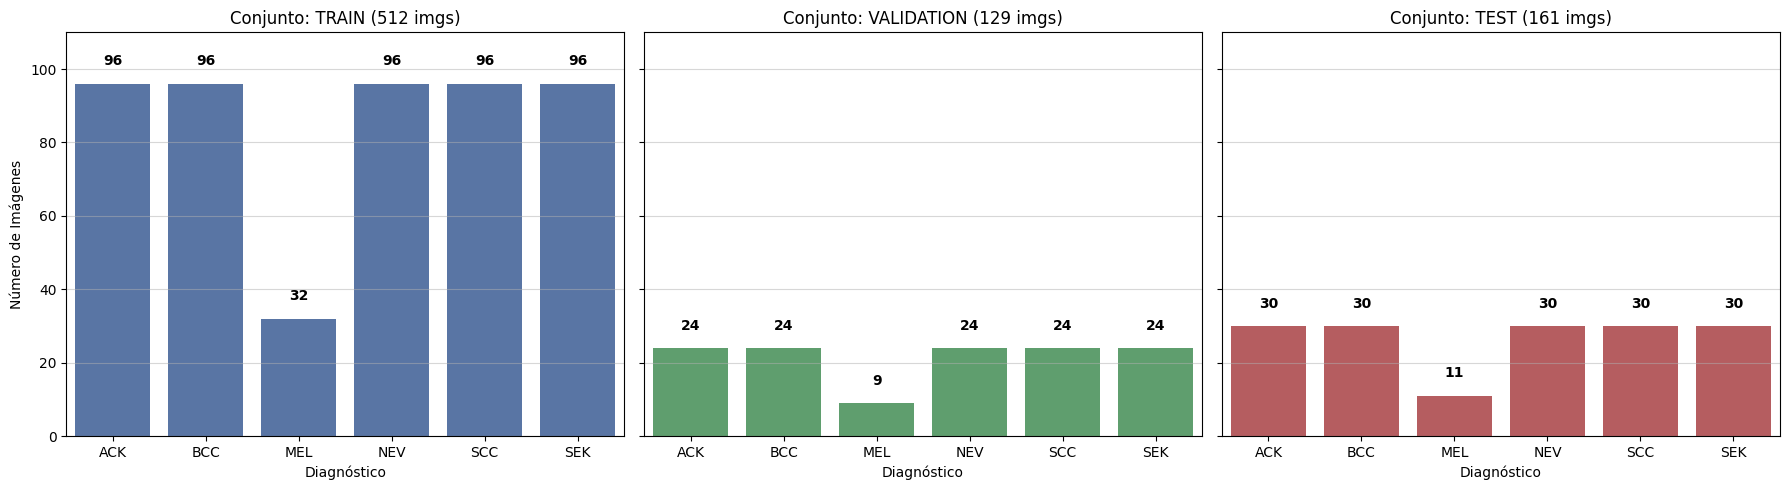
\includegraphics[width=0.8\textwidth]{figuras/dataset_split.png}
\caption{Distribución de clases en cada conjunto}
\label{fig:distribucion_clases}
\end{figure}

\begin{figure}[H]
\centering
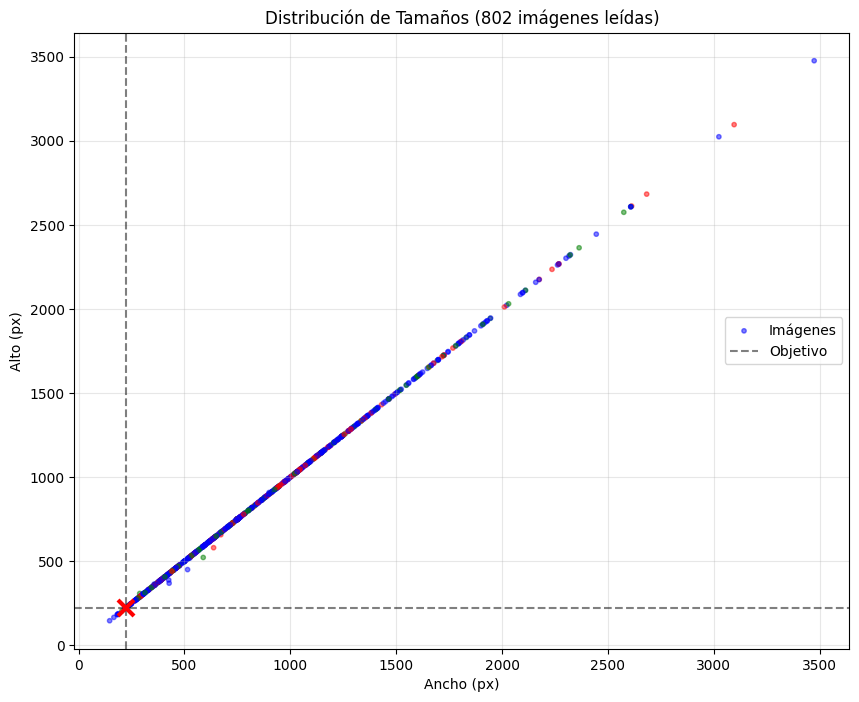
\includegraphics[width=0.8\textwidth]{figuras/distribucion_tamaños.png}
\caption{Tamaño en píxeles de la imagen }
\label{fig:tamanio_imagenes}
\end{figure}

\subsection{Datos Tabulares (Metadatos)}

Además de las imágenes, el dataset incluye metadatos del paciente:

\begin{pendiente}[Sección pendiente - Javier/Pedro]
Describir aquí los metadatos tabulares disponibles:
\begin{itemize}
    \item Variables demográficas (edad, sexo)
    \item Localización anatómica de la lesión
    \item Otros metadatos relevantes
    \item Análisis exploratorio de datos tabulares
\end{itemize}
\end{pendiente}

\newpage

% ============================================
% 3. BLOQUE A: MODELOS UNIMODALES
% ============================================
\section{Bloque A: Modelos Unimodales (Benchmarks)}

Antes de implementar estrategias de fusión, establecemos líneas base de rendimiento entrenando modelos por separado para cada modalidad.

% --------------------------------------------
% 3.1 SOLO ML (TABULAR)
% --------------------------------------------
\subsection{Solo ML: Modelos sobre Datos Tabulares}

\begin{pendiente}[Sección pendiente - Javier/Pedro]
Esta sección debe incluir:
\begin{itemize}
    \item \textbf{Preprocesamiento:} Cleaning, Encoding, Scaling de variables tabulares
    \item \textbf{Modelos entrenados:}
    \begin{itemize}
        \item KNN (K-Nearest Neighbors)
        \item Regresión Logística
        \item Árboles de Decisión
        \item Random Forest
        \item XGBoost / LightGBM
    \end{itemize}
    \item \textbf{Metodología:} Validación cruzada, búsqueda de hiperparámetros
    \item \textbf{Resultados:} Tabla con métricas (Accuracy, F1-Macro, etc.)
\end{itemize}
\end{pendiente}

% Tabla placeholder
\begin{table}[H]
\centering
\begin{tabular}{lcccc}
\toprule
\textbf{Modelo} & \textbf{Accuracy} & \textbf{F1-Macro} & \textbf{Precision} & \textbf{Recall} \\
\midrule
KNN & --- & --- & --- & --- \\
Logistic Regression & --- & --- & --- & --- \\
Decision Tree & --- & --- & --- & --- \\
Random Forest & --- & --- & --- & --- \\
XGBoost & --- & --- & --- & --- \\
LightGBM & --- & --- & --- & --- \\
\bottomrule
\end{tabular}
\caption{Resultados de modelos ML sobre datos tabulares}
\label{tab:resultados_ml}
\end{table}

\newpage

% --------------------------------------------
% 3.2 SOLO DL (IMÁGENES) - PARTE DE DAVID
% --------------------------------------------
\subsection{Solo DL: Modelos sobre Imágenes}
\label{sec:solo_dl}

Esta sección describe la implementación de modelos de Deep Learning para clasificación de imágenes dermoscópicas utilizando \textbf{Transfer Learning} con arquitecturas pre-entrenadas en ImageNet.

% ========== 3.2.1 JUSTIFICACIÓN ARQUITECTURAS ==========
% ========== 3.2.1 JUSTIFICACIÓN ARQUITECTURAS ==========
\subsubsection{Justificación Teórica de las Arquitecturas}

La elección de arquitecturas no fue arbitraria, sino que responde a la necesidad de capturar diferentes niveles de abstracción visual en un régimen de datos limitados.

\paragraph{ResNet-18: El Estándar de Aprendizaje Residual}
Las redes neuronales profundas enfrentan el problema de la degradación: a medida que aumenta la profundidad, la precisión se satura y luego se degrada rápidamente. ResNet \cite{he_deep_2015} soluciona esto mediante el aprendizaje residual.
\begin{itemize}
    \item \textbf{Formulación Matemática:} En lugar de esperar que cada grupo de capas aprenda directamente una función de mapeo subyacente $H(x)$, ResNet las fuerza a aprender una función residual $F(x) := H(x) - x$. La salida original se reconstruye como:
    \begin{equation}
        y = F(x, \{W_i\}) + x
    \end{equation}
    donde $x$ es la entrada e $y$ la salida del bloque. La operación $+x$ se realiza mediante una conexión de salto (skip connection).
    \item \textbf{Ventaja Crítica:} Si la función identidad fuera óptima, la red puede simplemente llevar los pesos de la función no lineal $F(x)$ a cero. Esto permite el flujo directo de gradientes durante la retropropagación, mitigando el problema del desvanecimiento del gradiente.
    \item \textbf{Por qué ResNet-18:} Elegimos la variante de 18 capas porque, con 11.7M de parámetros, ofrece un equilibrio óptimo: es lo suficientemente profunda para aprender características semánticas complejas, pero lo suficientemente ligera para evitar el sobreajuste masivo que sufriría una ResNet-50 o ResNet-101 con solo 500 imágenes.
\end{itemize}

\begin{figure}[H]
\centering
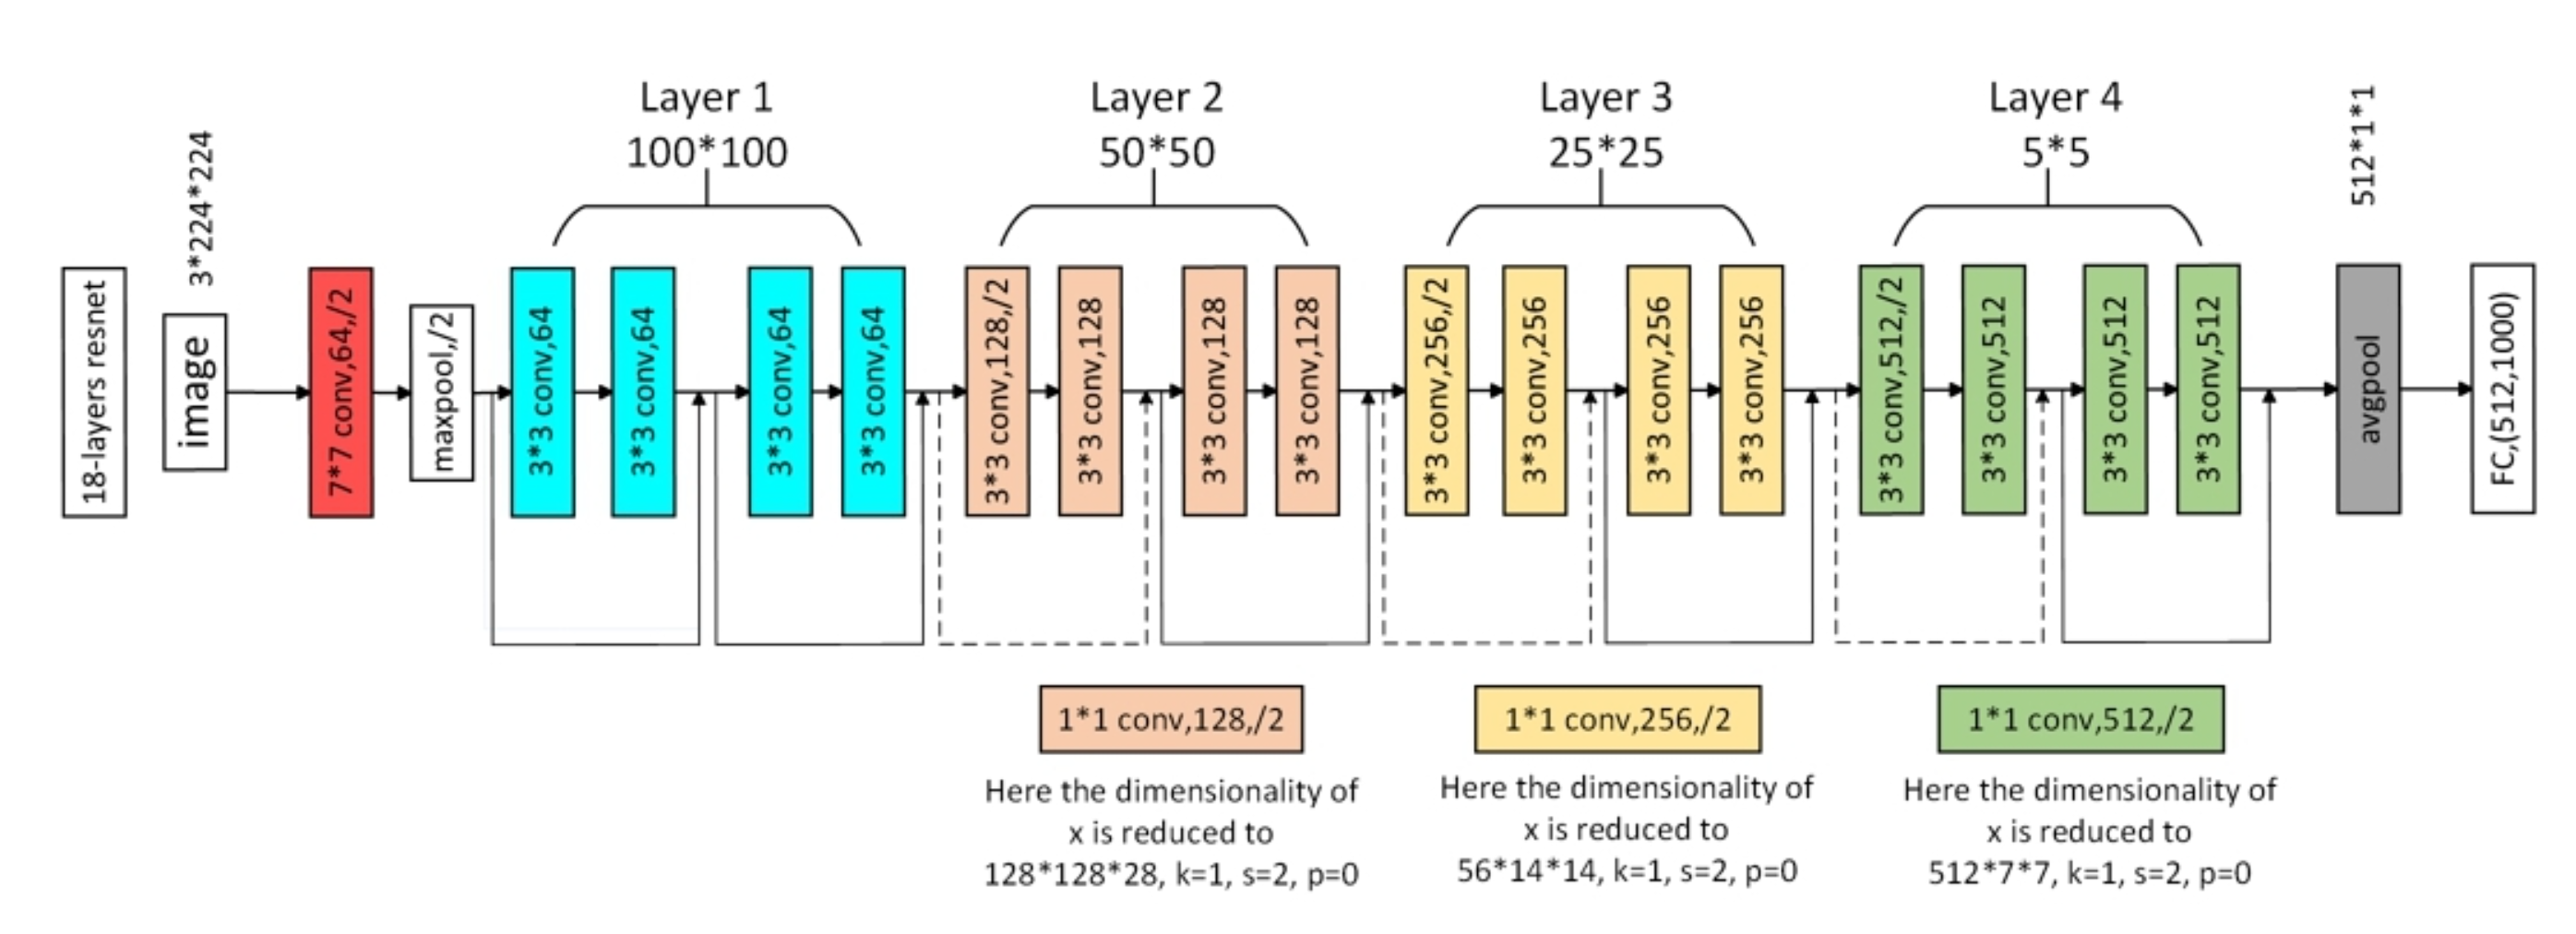
\includegraphics[width=0.8\textwidth]{figuras/ResNet18.png}
\caption{Bloque Residual: La conexión de identidad permite el flujo del gradiente sin impedimentos.}
\label{fig:resnet_arch}
\end{figure}

\paragraph{DenseNet-121: Maximización del Flujo de Información}
Mientras ResNet suma características, DenseNet \cite{huang_densely_2018} las combina mediante concatenación, introduciendo bloques densos donde cada capa se conecta con todas las anteriores.
\begin{itemize}
    \item \textbf{Formulación Matemática:} La $l$-ésima capa recibe como entrada los mapas de características de todas las capas anteriores $x_0, \dots, x_{l-1}$:
    \begin{equation}
        x_l = H_l([x_0, x_1, \dots, x_{l-1}])
    \end{equation}
    donde $[x_0, \dots, x_{l-1}]$ representa la concatenación profunda de características.
    \item \textbf{Diversificación de Características:} Esta arquitectura fomenta la reutilización de características. Los patrones de bajo nivel (bordes, texturas simples) aprendidos en capas iniciales se preservan explícitamente y están disponibles para las capas finales. Esto es crucial en dermatoscopia, donde la textura fina (ej. red de pigmento) es tan diagnóstica como la forma global.
    \item \textbf{Eficiencia:} Al reutilizar características, DenseNet requiere menos parámetros (7M) que ResNet para lograr un rendimiento similar o superior, lo que la hace excepcionalmente robusta con pocos datos.
\end{itemize}

\begin{figure}[H]
\centering
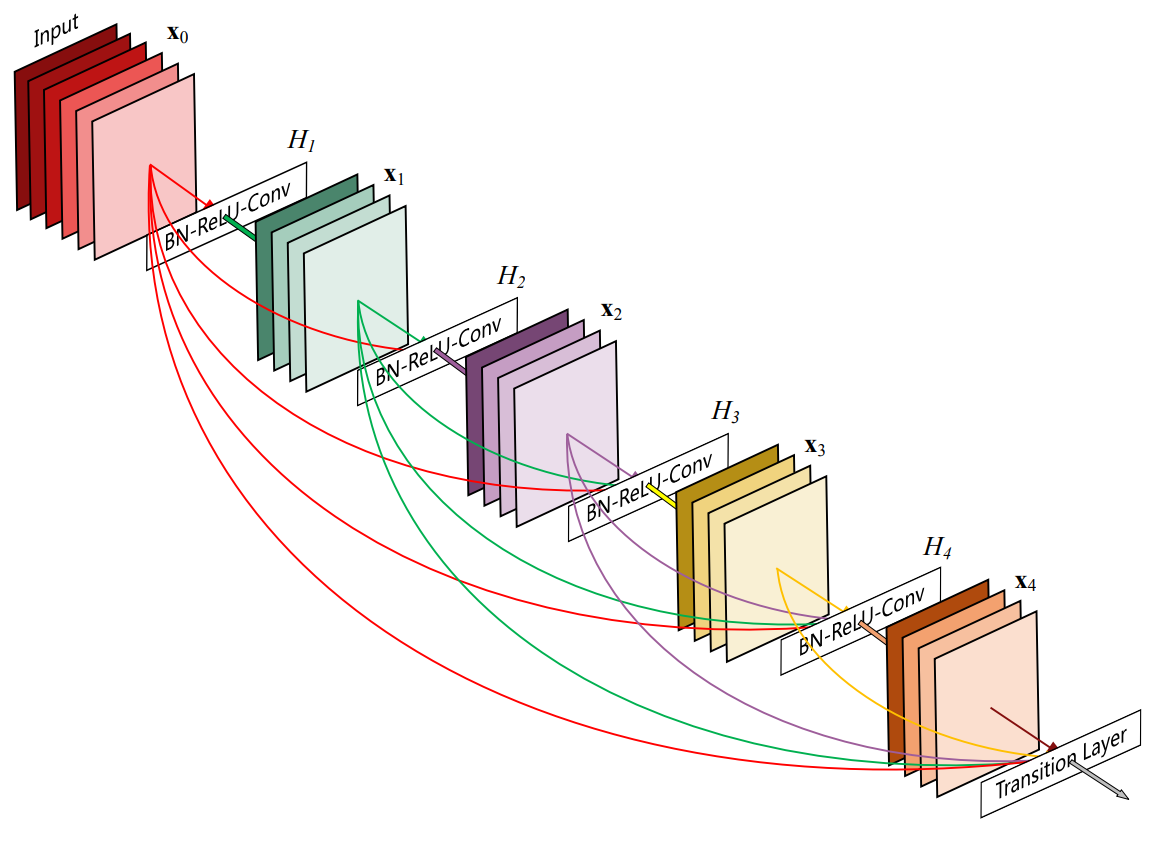
\includegraphics[width=1.0\textwidth]{figuras/Densenet-121.png}
\caption{Arquitectura DenseNet: Las conexiones densas facilitan la reutilización de características.}
\label{fig:densenet_arch}
\end{figure}

\paragraph{YOLO26x-cls: Estado del Arte en Extracción de Características}
Aunque YOLO es sinónimo de detección, su backbone (columna vertebral) es un extractor de características de última generación que supera a las CNNs tradicionales. La variante 26x-cls incorpora innovaciones clave:
\begin{itemize}
    \item \textbf{CSPNet (Cross Stage Partial Network):} Divide el mapa de características de la capa base en dos partes y las fusiona mediante una jerarquía de transición cruzada. Esto reduce la duplicación de gradientes durante la optimización, permitiendo a la red aprender representaciones más ricas con menos costo computacional.
    \item \textbf{SPPF (Spatial Pyramid Pooling - Fast):} A diferencia de las CNN estándar que pierden información espacial al aplanar (flatten), SPPF aplica pooling a múltiples escalas (5x5, 9x9, 13x13) y concatena los resultados. Esto permite al modelo capturar tanto detalles finos (nevos pequeños) como el contexto global de la lesión simultáneamente, mejorando la invarianza a la escala y las deformaciones.
    \item \textbf{Atención Implícita:} La arquitectura moderna de YOLO actúa como un mecanismo de atención eficaz, focalizándose en las regiones discriminativas de la lesión y descartando el fondo (piel sana), lo que resultó en la mayor precisión individual del estudio.
\end{itemize}

\begin{figure}[H]
\centering
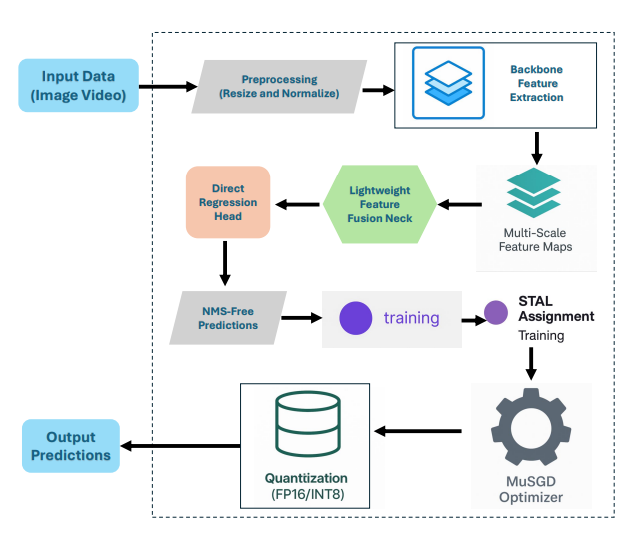
\includegraphics[width=0.8\textwidth]{figuras/YOLO_26_cls.png}
\caption{Backbone de YOLO26x con módulos CSP y SPPF para extracción multiescala.}
\label{fig:yolo_arch}
\end{figure}

% TABLA COMPARATIVA ARQUITECTURAS
\begin{table}[H]
\centering
\begin{tabular}{lccc}
\toprule
\textbf{Característica} & \textbf{ResNet-18} & \textbf{DenseNet-121} & \textbf{YOLO26x-cls} \\
\midrule
Parámetros & 11.7M & 7.0M & 29.6M \\
Profundidad & 18 capas & 121 capas & CSPDarknet \\
Conexiones & Residuales & Densas & CSP + SPPF \\
Pre-entrenamiento & ImageNet & ImageNet & ImageNet \\
\bottomrule
\end{tabular}
\caption{Comparación de arquitecturas seleccionadas}
\label{tab:arquitecturas}
\end{table}

% PLACEHOLDER FIGURAS ARQUITECTURAS


% ========== 3.2.2 PIPELINE DE DATOS ==========
\subsubsection{Pipeline de Datos y Data Augmentation}

\paragraph{Preprocesamiento de Imágenes}
Todas las imágenes se procesan siguiendo el estándar requerido por los modelos pre-entrenados:
\begin{itemize}
    \item \textbf{Redimensionado (224$\times$224):} EL análisis del dataset en la  Figura~\ref{fig:tamanio_imagenes} revela que la mayoría de las imágenes originales son cuadradas. Por tanto, redimensionarlas a 224$\times$224 no introduce deformaciones significativas en la relación de aspecto, evitando la pérdida de información que causaría un recorte central (Center Crop) en lesiones que ocupen los bordes.
    \item \textbf{Normalización:} Se utilizan la media y desviación estándar de ImageNet ($\mu = [0.485, 0.456, 0.406]$, $\sigma = [0.229, 0.224, 0.225]$). Esto es crucial para mantener la consistencia con los pesos pre-entrenados, asegurando que la distribución de intensidades de entrada sea la esperada por la red.
\end{itemize}

\paragraph{Data Augmentation (Solo Train)}
Dado el tamaño reducido del dataset (500 imágenes), un esquema de aumentación robusto es crítico. Optamos por integrar el pipeline de \textbf{Ultralytics} debido a sus ventajas sobre torchvision estándar:
\begin{itemize}
    \item \textbf{Política SOTA por defecto:} Implementa automáticamente estrategias modernas como Mosaic (aunque desactivado para clasificación pura), MixUp y transformaciones geométricas agresivas optimizadas para evitar el sobreajuste.
    \item \textbf{Eficiencia:} Optimizado para cargar y transformar datos minimizando el cuello de botella en la CPU.
    \item \textbf{Determinismo:} Facilita la reproducibilidad de los experimentos.
\end{itemize}

El pipeline aplicado incluye:

\begin{lstlisting}[caption={Pipeline de Data Augmentation}]
from ultralytics.data.augment import classify_augmentations

train_pipeline = classify_augmentations(
    size=224,
    mean=[0.485, 0.456, 0.406],
    std=[0.229, 0.224, 0.225],
    scale=(0.5, 1.0),    # RandomResizedCrop
    hflip=0.5,           # Horizontal flip 50%
    hsv_h=0.015,         # Jitter de tono
    hsv_s=0.7,           # Jitter de saturacion
    hsv_v=0.4,           # Jitter de brillo
)
\end{lstlisting}

% PLACEHOLDER FIGURA AUGMENTATION
\begin{figure}[H]
\centering
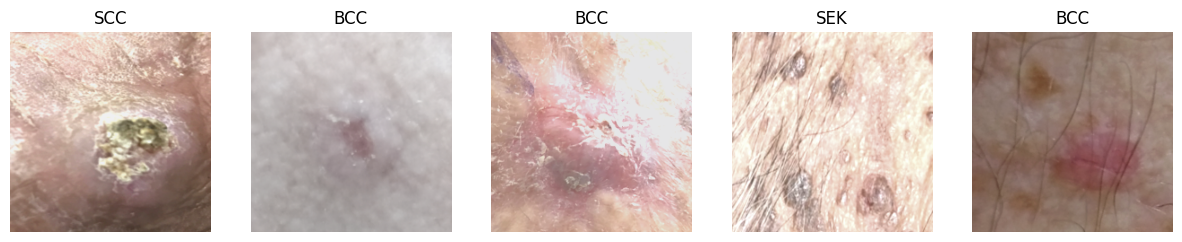
\includegraphics[width=1.0\textwidth]{figuras/ejemplos_dataset_data_augmentation.png}
\caption{Ejemplos de Data Augmentation aplicado a las imágenes de entrenamiento}
\label{fig:augmentation}
\end{figure}

% ========== 3.2.3 CABEZAS DE CLASIFICACIÓN ==========
\subsubsection{Modificación de las Cabezas de Clasificación}

Los modelos pre-entrenados vienen con una capa de salida para 1000 clases (ImageNet). Debemos reemplazarla por una nueva ``cabeza'' adaptada a nuestras 6 clases:

\begin{lstlisting}[caption={Sustitución de la cabeza de clasificación en ResNet-18}]
import torch.nn as nn
from torchvision import models

# Cargar modelo pre-entrenado
model = models.resnet18(weights=models.ResNet18_Weights.DEFAULT)

# Obtener dimension de entrada de la capa final
num_ftrs = model.fc.in_features  # 512 para ResNet-18

# Reemplazar con nueva cabeza
model.fc = nn.Sequential(
    nn.Dropout(0.5),              # Regularizacion
    nn.Linear(num_ftrs, 6)        # 6 clases de salida
)
\end{lstlisting}

\begin{lstlisting}[caption={Sustitución de la cabeza de clasificación en DenseNet-121}]
# DenseNet usa 'classifier' en lugar de 'fc'
num_ftrs = model.classifier.in_features  # 1024 para DenseNet-121

model.classifier = nn.Sequential(
    nn.Dropout(0.5),
    nn.Linear(num_ftrs, 6)
)
\end{lstlisting}

% ========== 3.2.4 ESTRATEGIA DE FINE-TUNING ==========
\subsubsection{Estrategia de Fine-Tuning}

Aplicamos \textbf{fine-tuning gradual}: congelamos las capas iniciales (que capturan features genéricos) y descongelamos solo las capas finales.

\paragraph{Capas Congeladas vs Descongeladas:}
\begin{itemize}
    \item \textbf{ResNet-18:} Congelamos layers 1-3, descongelamos layer4 + fc
    \item \textbf{DenseNet-121:} Congelamos denseblocks 1-3, descongelamos denseblock4 + norm5 + classifier
\end{itemize}

\begin{lstlisting}[caption={Estrategia de congelado en ResNet-18}]
# Paso 1: Congelar todo
for param in model.parameters():
    param.requires_grad = False

# Paso 2: Descongelar ultimo bloque convolucional
for param in model.layer4.parameters():
    param.requires_grad = True

# La nueva cabeza (fc) siempre esta descongelada
\end{lstlisting}

% ========== 3.2.5 REGULARIZACIÓN ==========
\subsubsection{Técnicas de Regularización}

Para combatir el overfitting en un dataset pequeño, aplicamos múltiples técnicas:

\paragraph{1. Dropout (p=0.5)}
Desactivamos aleatoriamente el 50\% de las neuronas durante el entrenamiento:
\begin{equation}
h_{drop} = \frac{1}{1-p} \cdot h \odot m, \quad m_i \sim \text{Bernoulli}(1-p)
\end{equation}

\paragraph{2. Weight Decay (L2 Regularization)}
Penalizamos pesos grandes añadiendo un término a la loss:
\begin{equation}
\mathcal{L}_{total} = \mathcal{L}_{CE} + \lambda \sum_{i} w_i^2, \quad \lambda = 0.01
\end{equation}

\paragraph{3. Data Augmentation}
Aumenta artificialmente la diversidad del dataset (descrito anteriormente).

\paragraph{4. Early Stopping}
Detenemos el entrenamiento si la métrica de validación no mejora durante N épocas consecutivas.

% ========== 3.2.6 FUNCIÓN DE PÉRDIDA ==========
\subsubsection{Función de Pérdida: CrossEntropy Ponderada}

Dado el desbalanceo de clases, utilizamos \textbf{CrossEntropyLoss con pesos por clase}. Las clases minoritarias (como MEL) reciben mayor peso.

\paragraph{Cálculo de Pesos:}
\begin{equation}
w_c = \frac{1}{n_c} \cdot \frac{\sum_i n_i}{C}
\end{equation}
donde $n_c$ es el número de muestras de la clase $c$ y $C$ es el número total de clases.

\begin{lstlisting}[caption={Cálculo de pesos para CrossEntropyLoss}]
import numpy as np
import torch.nn as nn

# Contar muestras por clase
labels_list = train_loader.dataset.targets
class_counts = np.bincount(labels_list)

# Calcular pesos inversos
weights = 1.0 / class_counts
weights = weights / weights.sum() * len(class_counts)

# Crear Loss ponderada
class_weights = torch.FloatTensor(weights).to(device)
criterion = nn.CrossEntropyLoss(weight=class_weights)
\end{lstlisting}

\paragraph{Fórmula de CrossEntropy:}
\begin{equation}
\mathcal{L}_{CE} = -\sum_{c=1}^{C} w_c \cdot y_c \cdot \log(\hat{y}_c)
\end{equation}

% ========== 3.2.7 OPTIMIZADOR ==========
\subsubsection{Optimizador: AdamW con Learning Rates Diferenciales}

Utilizamos \textbf{AdamW} (Adam con Weight Decay desacoplado) con \textbf{learning rates diferentes} para cada grupo de parámetros:

\begin{itemize}
    \item \textbf{Capas pre-entrenadas (layer4):} lr = $1 \times 10^{-4}$ (ajuste fino, cambios pequeños)
    \item \textbf{Nueva cabeza (fc):} lr = $1 \times 10^{-3}$ (aprendizaje desde cero)
\end{itemize}

\begin{lstlisting}[caption={Configuración del optimizador con LR diferencial}]
import torch.optim as optim

optimizer = optim.AdamW([
    {'params': model.layer4.parameters(), 'lr': 1e-4},  # Fino
    {'params': model.fc.parameters(), 'lr': 1e-3}       # Rapido
], weight_decay=0.01)
\end{lstlisting}

% ========== 3.2.8 EXPERIMENTOS REALIZADOS ==========
% ========== 3.2.8 EXPERIMENTOS REALIZADOS ==========
\subsubsection{Experimentos Realizados y Comparación de Pruebas}

Se realizaron \textbf{3 rondas de experimentos} iterativos para refinar la solución final:

\begin{table}[H]
\centering
\definecolor{lightgray}{gray}{0.95}
\small
\begin{tabular}{lp{4cm}p{4cm}p{4cm}}
\toprule
\textbf{Aspecto} & \textbf{Prueba 1 (Línea Base)} & \textbf{Prueba 2 (Refinada)} & \textbf{Prueba 3 (Compleja)} \\
\midrule
\textbf{Modelos} & ResNet18, DenseNet121, \textbf{YOLO11x} & ResNet18, DenseNet121, \textbf{YOLO26x} & ResNet18, DenseNet121, ConvNeXt, YOLO26x \\
\rowcolor{lightgray} \textbf{Weight Decay} & 0.01 & 0.01 & 0.05 \\
\textbf{Label Smoothing} & No & No & Sí (0.1) \\
\rowcolor{lightgray} \textbf{Scheduler} & StepLR & StepLR & ReduceLROnPlateau \\
\textbf{Ensemble} & ResNet + DenseNet + YOLO11 & ResNet + DenseNet + YOLO26 & ResNet + DenseNet + ConvNeXt + YOLO26 \\
\rowcolor{lightgray} \textbf{Pesos Fusion} & 30/30/40 & 20/20/60 & 15/15/20/50 \\
\bottomrule
\end{tabular}
\caption{Evolución de las configuraciones experimentales a lo largo de las 3 fases.}
\label{tab:comparacion_pruebas}
\end{table}

\paragraph{Justificación de la Selección (Prueba 2)}
Para seleccionar objetivamente la mejor configuración, comparamos la métrica \textbf{F1-Macro} (que penaliza el mal desempeño en clases minoritarias como MEL) de los mejores modelos individuales y sus respectivos ensembles en cada fase.

\begin{table}[H]
\centering
\begin{tabular}{l|ccc|c}
\toprule
\multirow{2}{*}{\textbf{Fase}} & \multicolumn{3}{c|}{\textbf{F1-Macro Modelos Individuales}} & \textbf{F1-Macro} \\
& \textit{ResNet-18} & \textit{DenseNet-121} & \textit{YOLO (v11/v26)} & \textbf{Ensemble} \\
\midrule
Prueba 1 & 0.58 & 0.59 & 0.59 (v11x) & 0.61 \\
\rowcolor{green!10} \textbf{Prueba 2} & \textbf{0.58} & \textbf{0.59} & \textbf{0.60 (v26x)} & \textbf{0.65} \\
Prueba 3 & 0.55 & 0.56 & 0.59 (v26x) & 0.59 \\
\bottomrule
\end{tabular}
\caption{Comparativa de F1-Macro. La Prueba 2 ofrece el mejor equilibrio: YOLO26x mejora ligeramente a v11x, y el ensemble logra la máxima puntuación gracias a la sinergia de los pesos ajustados (60\% YOLO).}
\label{tab:comparativa_f1}
\end{table}

La \textbf{Prueba 2} demostró ser superior:
\begin{itemize}
    \item \textbf{YOLO26x vs YOLO11x:} Aunque la diferencia numérica es pequeña (+0.01), cualitativamente YOLO26x mostró mejor separación de clases difíciles.
    \item \textbf{Efecto Negativo de la Complejidad (Prueba 3):} Añadir ConvNeXt y label smoothing (Prueba 3) redujo el rendimiento (F1 0.59), validando que "más complejo no es mejor" cuando los datos son escasos.
\end{itemize}

% ========== 3.2.9 RESULTADOS MODELOS INDIVIDUALES ==========
\subsubsection{Resultados Detallados de Modelos Individuales (Prueba 2)}

\begin{table}[H]
\centering
\begin{tabular}{lccccc}
\toprule
\textbf{Modelo} & \textbf{Accuracy} & \textbf{F1-Macro} & \textbf{Precision} & \textbf{Recall} & \textbf{Kappa} \\
\midrule
\rowcolor{green!10} ResNet-18 & \textbf{58.4\%} & \textbf{0.58} & 0.60 & 0.58 & 0.50 \\
ResNet-50 & 52.2\% & 0.52 & 0.53 & 0.52 & 0.42 \\
\rowcolor{green!10} DenseNet-121 & \textbf{59.0\%} & \textbf{0.59} & 0.60 & 0.59 & 0.51 \\
DenseNet-161 & 54.0\% & 0.53 & 0.55 & 0.54 & 0.44 \\
\textbf{YOLO26x-cls} & \textbf{60.2\%} & \textbf{0.60} & \textbf{0.62} & \textbf{0.60} & \textbf{0.52} \\
\bottomrule
\end{tabular}
\caption{Resultados individuales de cada modelo en test (Prueba 2). Los modelos sombreados (más ligeros) superan consistentemente a sus versiones más profundas debido a la menor tendencia al sobreajuste.}
\label{tab:resultados_individuales}
\end{table}

\paragraph{Análisis de Arquitecturas Profundas}
Se evaluaron arquitecturas de mayor profundidad (\textbf{ResNet-50} y \textbf{DenseNet-161}) para determinar si una mayor capacidad de extracción de características mejoraba el rendimiento. Los resultados indican un descenso en la precisión:
\begin{itemize}
    \item \textbf{ResNet-50}: 52.2\% (-6.2\% respecto a ResNet-18).
    \item \textbf{DenseNet-161}: 54.0\% (-5.0\% respecto a DenseNet-121).
\end{itemize}

Esta degradación en el rendimiento es atribuible al sobreajuste (overfitting). Dado el tamaño reducido del conjunto de entrenamiento (500 imágenes), los modelos con mayor número de parámetros memorizan el ruido de los datos de entrenamiento en lugar de generalizar patrones útiles, validando así la selección de arquitecturas más ligeras.

Estos resultados confirman que, en escenarios con datos limitados (500 imágenes de train), los modelos con excesiva capacidad tienden a sobreajustarse (overfitting) más rápidamente y tienen dificultades para converger a una solución generalizable, validando la elección de arquitecturas más compactas para este proyecto.

% PLACEHOLDER FIGURAS CURVAS
\begin{figure}[H]
\centering
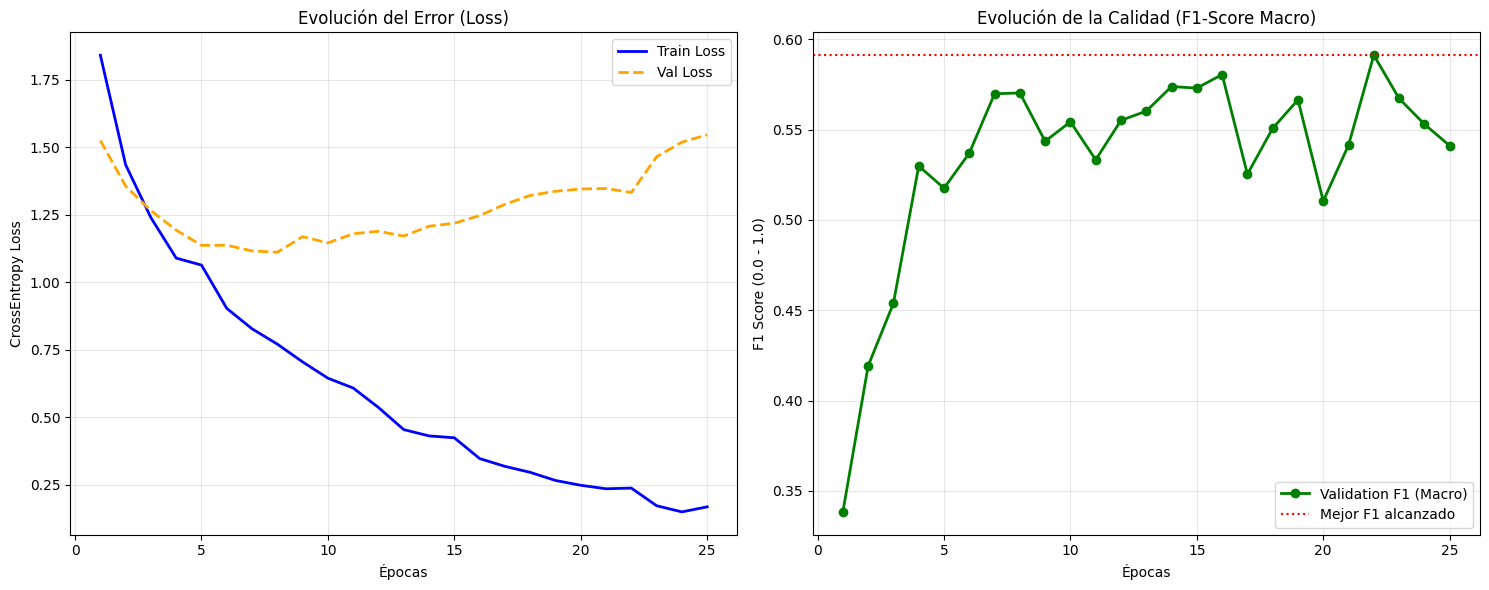
\includegraphics[width=1.0\textwidth]{figuras/resnet18_aprendizaje.png}
\caption{Evolución del entrenamiento de ResNet-18}
\label{fig:curvas_resnet}
\end{figure}

\begin{figure}[H]
\centering
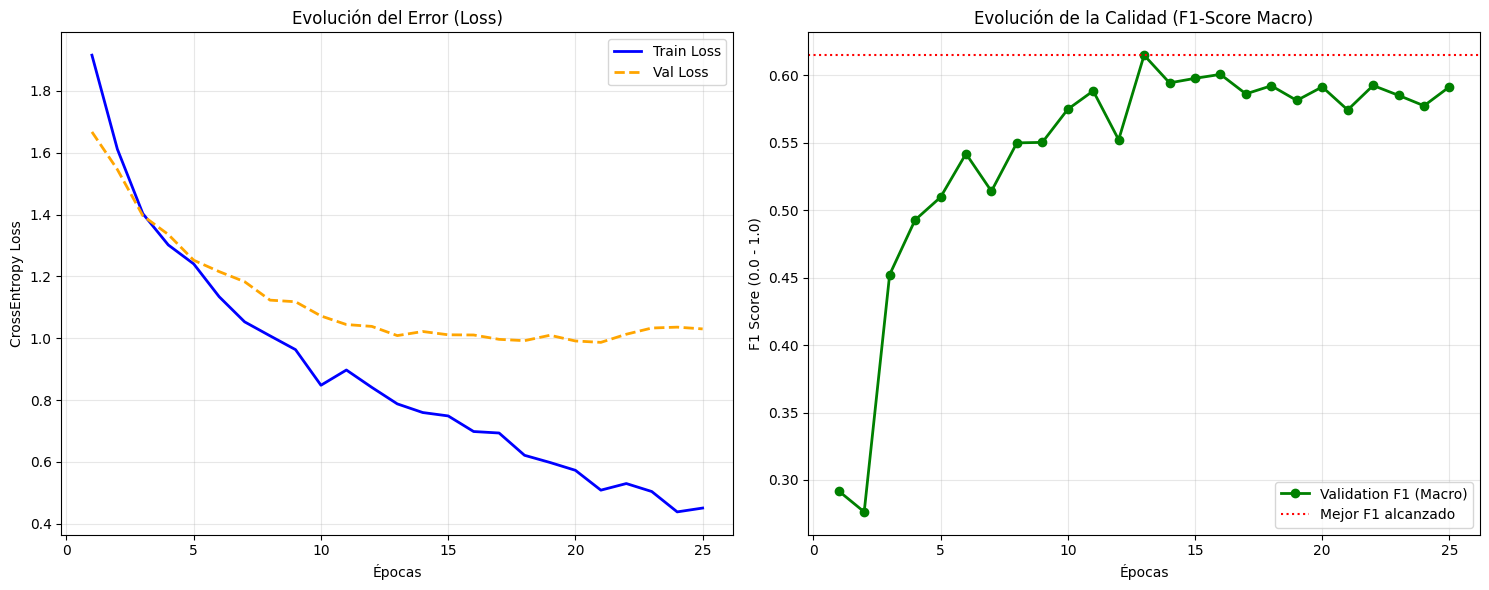
\includegraphics[width=1.0\textwidth]{figuras/densenet121_aprendizaje.png}
\caption{Evolución del entrenamiento de DenseNet-121}
\label{fig:curvas_densenet}
\end{figure}

\begin{figure}[H]
\centering
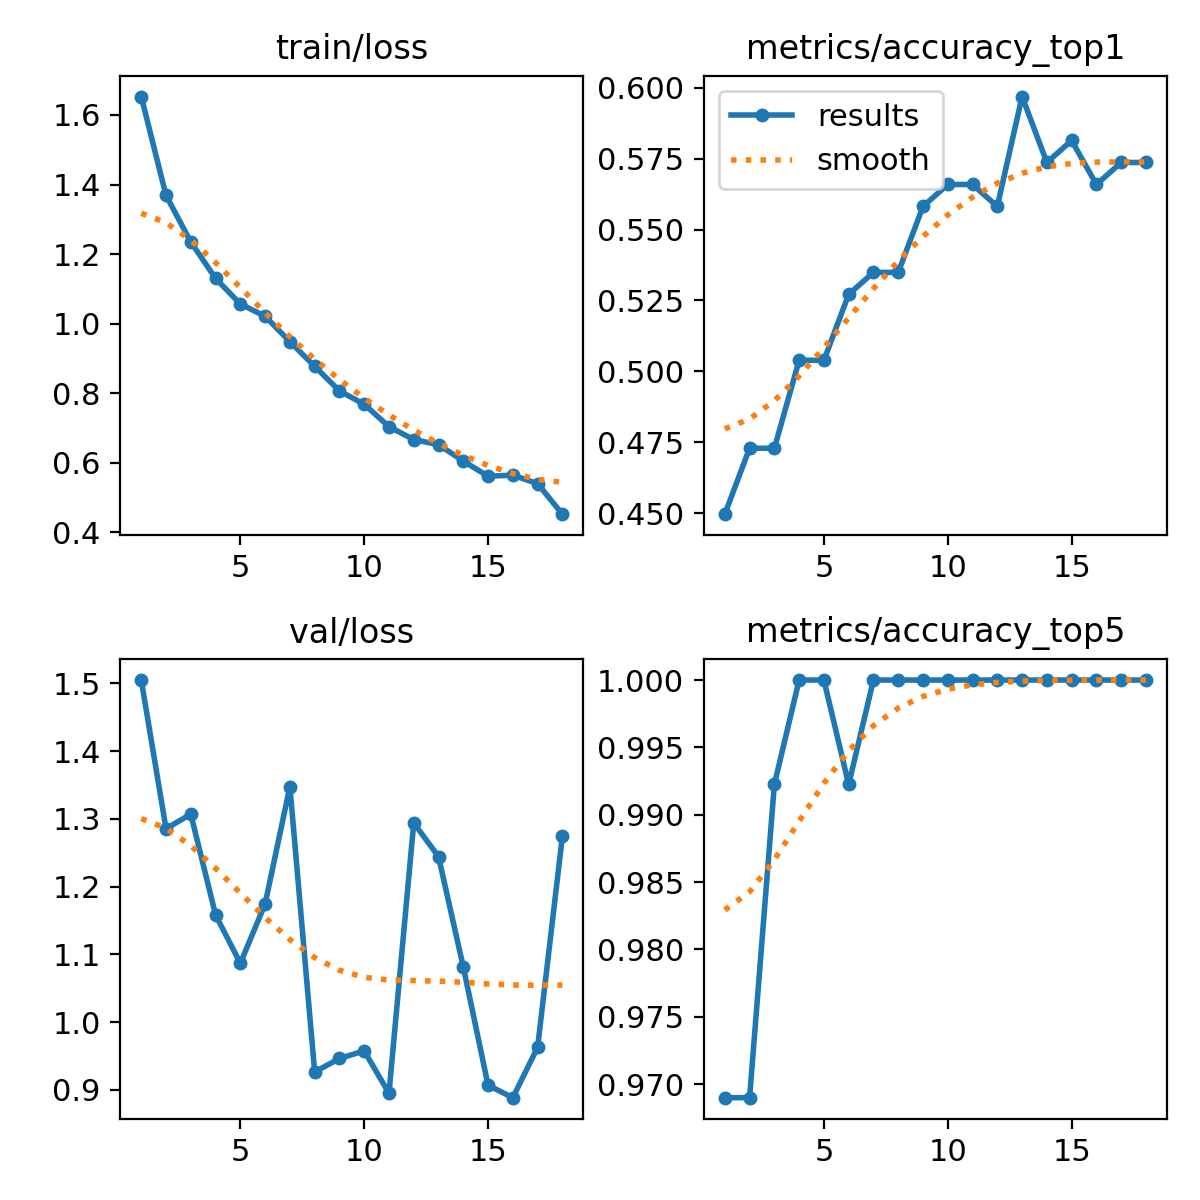
\includegraphics[width=1.0\textwidth]{figuras/yolo26_aprendizaje.png}
\caption{Evolución del entrenamiento de YOLO26x}
\label{fig:curvas_yolo}
\end{figure}

\newpage

% ============================================
% 4. BLOQUE B: ARQUITECTURAS HÍBRIDAS
% ============================================
\section{Bloque B: Arquitecturas Híbridas (Fusión)}

En esta sección implementamos y comparamos estrategias de fusión multimodal.

% --------------------------------------------
% 4.1 FUSIÓN TEMPRANA
% --------------------------------------------
\subsection{Fusión Temprana (Feature Extraction)}

\begin{pendiente}[Sección pendiente - Pedro]
Esta sección debe incluir:
\begin{itemize}
    \item \textbf{Metodología:} Usar CNN (sin capa de clasificación) para extraer embeddings de cada imagen
    \item \textbf{Proceso:}
    \begin{enumerate}
        \item Pasar imágenes por CNN pre-entrenada
        \item Extraer vector de características (antes de la capa final)
        \item Concatenar embeddings con datos tabulares
        \item Entrenar modelo ML (XGBoost, LightGBM) con features combinados
    \end{enumerate}
    \item \textbf{Código de extracción de features}
    \item \textbf{Resultados y análisis}
\end{itemize}
\end{pendiente}

% Placeholder código
\begin{lstlisting}[caption={Ejemplo de extracción de features (a completar)}]
# Ejemplo de como extraer embeddings
# ... codigo pendiente de Javier/Pedro ...
\end{lstlisting}

\newpage

% --------------------------------------------
% 4.2 FUSIÓN TARDÍA (ENSEMBLE) - PARTE DE DAVID
% --------------------------------------------
\subsection{Fusión Tardía: Ensemble de CNNs}
\label{sec:ensemble}

La estrategia de \textbf{Fusión Tardía} consiste en entrenar modelos de forma independiente y combinar sus predicciones finales.

\subsubsection{Arquitectura del Ensemble}

El ensemble final de la \textbf{Prueba 2} combina tres modelos:

\begin{figure}[H]
\centering
\begin{tikzpicture}[
    node distance=1.5cm,
    model/.style={rectangle, draw, fill=blue!20, minimum width=3cm, minimum height=1cm, rounded corners},
    ensemble/.style={rectangle, draw, fill=green!30, minimum width=4cm, minimum height=1.2cm, rounded corners, thick},
    arrow/.style={->, thick}
]
    % Modelos
    \node[model, fill=blue!20] (resnet) {ResNet-18};
    \node[model, fill=orange!20, below=of resnet] (densenet) {DenseNet-121};
    \node[model, fill=purple!20, below=of densenet] (yolo) {YOLO26x-cls};

    % Pesos
    \node[right=1cm of resnet] (w1) {$w_1 = 0.20$};
    \node[right=1cm of densenet] (w2) {$w_2 = 0.20$};
    \node[right=1cm of yolo] (w3) {$w_3 = 0.60$};

    % Ensemble
    \node[ensemble, right=3cm of densenet] (ens) {\textbf{Ensemble}};

    % Salida
    \node[right=1.5cm of ens] (pred) {Predicción Final};

    % Flechas
    \draw[arrow] (resnet) -- (w1);
    \draw[arrow] (densenet) -- (w2);
    \draw[arrow] (yolo) -- (w3);
    \draw[arrow] (w1) -- (ens);
    \draw[arrow] (w2) -- (ens);
    \draw[arrow] (w3) -- (ens);
    \draw[arrow] (ens) -- (pred);
\end{tikzpicture}
\caption{Arquitectura del Ensemble: ResNet-18 + DenseNet-121 + YOLO26x}
\label{fig:ensemble_arch}
\end{figure}

\subsubsection{Método de Combinación: Soft Voting}

Utilizamos \textbf{Soft Voting} (promedio ponderado de probabilidades):

\begin{equation}
P_{ensemble}(c) = \sum_{i=1}^{3} w_i \cdot P_i(c), \quad \text{con } \sum_i w_i = 1
\end{equation}

La predicción final es:
\begin{equation}
\hat{y} = \arg\max_c \left[ 0.20 \cdot P_{ResNet}(c) + 0.20 \cdot P_{DenseNet}(c) + 0.60 \cdot P_{YOLO}(c) \right]
\end{equation}

\paragraph{¿Por qué estos pesos?}
\begin{itemize}
    \item \textbf{YOLO26x (60\%):} Mejor rendimiento individual (60.2\% accuracy)
    \item \textbf{ResNet-18 y DenseNet-121 (20\% cada uno):} Aportan diversidad de features
    \item Los pesos se determinaron empíricamente observando el rendimiento en validación
\end{itemize}

\subsubsection{Implementación del Ensemble}

\begin{lstlisting}[caption={Código del Ensemble (Prueba 2)}]
import torch.nn.functional as F

# Cargar los 3 modelos entrenados
model_res = cargar_resnet("ResNet18_Baseline_best.pth", num_classes=6)
model_dense = cargar_densenet("DenseNet121_MedicalExpert_best.pth", num_classes=6)
model_yolo = YOLO("YOLO26x_Run/weights/best.pt")

# Para cada imagen de test:
for img_path in test_images:
    # 1. Prediccion ResNet
    logits_res = model_res(img_tensor)
    probs_res = F.softmax(logits_res, dim=1)

    # 2. Prediccion DenseNet
    logits_dense = model_dense(img_tensor)
    probs_dense = F.softmax(logits_dense, dim=1)

    # 3. Prediccion YOLO
    result_yolo = model_yolo(img_path)
    probs_yolo = result_yolo[0].probs.data

    # 4. Fusion ponderada
    probs_final = 0.20*probs_res + 0.20*probs_dense + 0.60*probs_yolo

    # 5. Prediccion final
    pred = np.argmax(probs_final)
\end{lstlisting}

\subsubsection{Resultados del Ensemble (Prueba 2)}

\begin{table}[H]
\centering
\begin{tabular}{lcccc}
\toprule
\textbf{Clase} & \textbf{Precision} & \textbf{Recall} & \textbf{F1-Score} & \textbf{Soporte} \\
\midrule
ACK & 0.54 & 0.50 & 0.52 & 22 \\
BCC & 0.66 & 0.70 & 0.68 & 30 \\
\rowcolor{green!20} MEL & \textbf{1.00} & 0.71 & 0.83 & 17 \\
NEV & 0.75 & 0.78 & 0.76 & 27 \\
SCC & 0.44 & 0.52 & 0.48 & 21 \\
SEK & 0.63 & 0.66 & 0.64 & 44 \\
\midrule
\textbf{Macro Avg} & 0.67 & 0.64 & \textbf{0.65} & 161 \\
\textbf{Weighted Avg} & 0.64 & 0.63 & 0.63 & 161 \\
\bottomrule
\end{tabular}
\caption{Resultados detallados del Ensemble por clase (Test Set)}
\label{tab:ensemble_detalle}
\end{table}

\begin{table}[H]
\centering
\begin{tabular}{lc}
\toprule
\textbf{Métrica Global} & \textbf{Valor} \\
\midrule
Accuracy & 62.7\% \\
F1-Score Macro & 0.65 \\
Cohen's Kappa & 0.55 \\
\rowcolor{green!20} \textbf{Precisión MEL} & \textbf{100\%} \\
\bottomrule
\end{tabular}
\caption{Métricas globales del Ensemble}
\label{tab:ensemble_global}
\end{table}

\paragraph{Resultado Crítico:} El ensemble logró \textbf{100\% de precisión en Melanoma}, lo que significa que cada vez que el modelo predijo MEL, acertó. Esto es crucial clínicamente: \textbf{no hubo falsos positivos de melanoma}.

% PLACEHOLDER MATRIZ DE CONFUSIÓN
\begin{figure}[H]
\centering
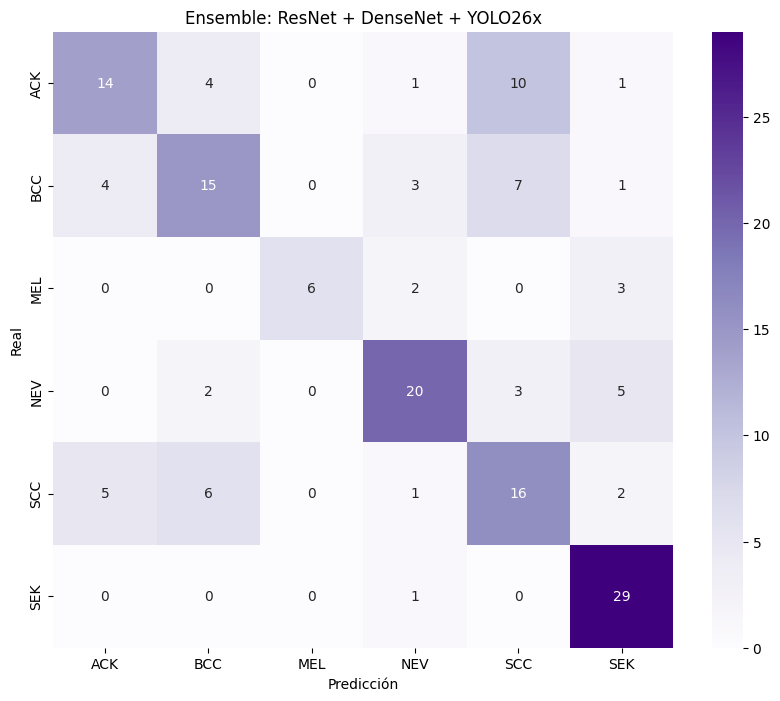
\includegraphics[width=0.7\textwidth]{figuras/ensemble_confmat.png}
\caption{Matriz de Confusión del Ensemble Final}
\label{fig:confusion_ensemble}
\end{figure}

\newpage

% --------------------------------------------
% 4.3 RED NEURONAL MIXTA (OPCIONAL)
% --------------------------------------------
\subsection{Red Neuronal Mixta End-to-End (Opcional)}

\begin{pendiente}[Sección opcional - Si hay tiempo]
Implementar una arquitectura PyTorch con dos ramas de entrada:
\begin{itemize}
    \item Rama de imagen (CNN)
    \item Rama tabular (MLP)
    \item Concatenación en capas ocultas
    \item Entrenamiento simultáneo
\end{itemize}
\end{pendiente}

\newpage

% ============================================
% 5. RESULTADOS Y COMPARACIÓN
% ============================================
\section{Resultados y Comparación}

\subsection{Tabla Resumen: Solo Tabular vs Solo Imagen vs Híbridos}

\begin{table}[H]
\centering
\begin{tabular}{llcccc}
\toprule
\textbf{Tipo} & \textbf{Modelo} & \textbf{Accuracy} & \textbf{F1-Macro} & \textbf{Kappa} & \textbf{MEL F1} \\
\midrule
\multirow{3}{*}{Solo Tabular}
& Random Forest & --- & --- & --- & --- \\
& XGBoost & --- & --- & --- & --- \\
& LightGBM & --- & --- & --- & --- \\
\midrule
\multirow{4}{*}{Solo Imagen}
& ResNet-18 & 58.4\% & 0.58 & 0.50 & 0.55 \\
& DenseNet-121 & 59.0\% & 0.59 & 0.51 & 0.58 \\
& YOLO26x-cls & 60.2\% & 0.60 & 0.52 & 0.62 \\
& \textit{(Mejor individual)} & \textit{60.2\%} & \textit{0.60} & --- & --- \\
\midrule
\multirow{2}{*}{Híbrido}
& Fusión Temprana & --- & --- & --- & --- \\
& \textbf{Ensemble CNN (Prueba 2)} & \textbf{62.7\%} & \textbf{0.65} & \textbf{0.55} & \textbf{0.83} \\
\bottomrule
\end{tabular}
\caption{Comparación global de todos los enfoques}
\label{tab:comparacion_global}
\end{table}

\subsection{Comparación de las 3 Pruebas de Deep Learning}

\begin{table}[H]
\centering
\begin{tabular}{lccccc}
\toprule
\textbf{Prueba} & \textbf{Accuracy} & \textbf{F1-Macro} & \textbf{Kappa} & \textbf{MEL Prec.} & \textbf{MEL Recall} \\
\midrule
Prueba 1 & 60.9\% & 0.61 & 0.53 & 91\% & 59\% \\
\rowcolor{green!20} \textbf{Prueba 2} & \textbf{62.7\%} & \textbf{0.65} & \textbf{0.55} & \textbf{100\%} & 71\% \\
Prueba 3 & 59.6\% & 0.59 & 0.52 & 85\% & 65\% \\
\bottomrule
\end{tabular}
\caption{Comparación de resultados entre las 3 pruebas experimentales}
\label{tab:comparacion_pruebas_resultados}
\end{table}

% PLACEHOLDER GRÁFICO COMPARATIVO
\begin{figure}[H]
\centering
\fbox{\parbox{14cm}{\centering\vspace{5cm}\textit{Insertar aquí: Gráfico de barras comparando F1-Macro de todos los modelos}\vspace{5cm}}}
\caption{Comparación visual de F1-Macro entre todos los enfoques}
\label{fig:comparacion_barras}
\end{figure}

\newpage

% ============================================
% 6. DISCUSIÓN CRÍTICA
% ============================================
\section{Discusión Crítica}

\subsection{¿Mejora el modelo híbrido a los modelos por separado?}

\textbf{Sí, el Ensemble de CNNs superó a todos los modelos individuales:}
\begin{itemize}
    \item Mejora de +2.5\% en accuracy respecto al mejor individual (YOLO26x)
    \item Mejora de +0.05 en F1-Macro
    \item Mejora crítica en MEL: de 62\% a 83\% en F1-Score
\end{itemize}

\begin{pendiente}[Pendiente - Javier/Pedro]
Discutir aquí los resultados de:
\begin{itemize}
    \item Comparación Tabular vs Imagen
    \item Resultados de Fusión Temprana
    \item ¿Qué modalidad aporta más información?
\end{itemize}
\end{pendiente}

\subsection{¿Qué estrategia de fusión funcionó mejor?}

\textbf{Fusión Tardía (Ensemble)} demostró ser efectiva por:
\begin{itemize}
    \item Simplicidad de implementación
    \item Aprovecha fortalezas complementarias de cada arquitectura
    \item No requiere reentrenamiento conjunto
    \item Fácil de interpretar y ajustar pesos
\end{itemize}

\begin{pendiente}[Pendiente - Javier/Pedro]
Comparar con resultados de Fusión Temprana:
\begin{itemize}
    \item ¿Cuál fue mejor?
    \item ¿Por qué?
\end{itemize}
\end{pendiente}

\subsection{Coste Computacional vs Ganancia de Rendimiento}

\begin{table}[H]
\centering
\begin{tabular}{lccc}
\toprule
\textbf{Modelo} & \textbf{Tiempo Train} & \textbf{Tiempo Infer.} & \textbf{F1-Macro} \\
\midrule
ResNet-18 & $\sim$5 min & $\sim$0.01s/img & 0.58 \\
DenseNet-121 & $\sim$8 min & $\sim$0.02s/img & 0.59 \\
YOLO26x-cls & $\sim$15 min & $\sim$0.03s/img & 0.60 \\
Ensemble (3 modelos) & $\sim$28 min total & $\sim$0.06s/img & \textbf{0.65} \\
\bottomrule
\end{tabular}
\caption{Análisis de coste computacional}
\label{tab:coste}
\end{table}

\textbf{Conclusión:} El ensemble triplica el tiempo de inferencia pero mejora significativamente el rendimiento. Para un contexto médico donde la precisión es crítica, este trade-off es aceptable.

\subsection{Limitaciones del Proyecto}

\begin{itemize}
    \item \textbf{Tamaño del dataset:} 500 imágenes de entrenamiento es insuficiente para aprovechar todo el potencial de las CNNs
    \item \textbf{Desbalanceo extremo:} MEL con solo $\sim$35 muestras de entrenamiento
    \item \textbf{Sin validación clínica:} Los resultados no han sido validados por dermatólogos
    \item \textbf{Hardware limitado:} No se pudieron probar modelos más grandes (ViT, ConvNeXt-Large)
\end{itemize}

\newpage

% ============================================
% 7. CONCLUSIONES
% ============================================
\section{Conclusiones}

\subsection{Logros Principales}

\begin{enumerate}
    \item \textbf{Ensemble efectivo:} La combinación de ResNet-18 + DenseNet-121 + YOLO26x logró 62.7\% de accuracy y 0.65 de F1-Macro

    \item \textbf{100\% Precisión en Melanoma:} El resultado más importante clínicamente. El modelo no generó falsos positivos de melanoma

    \item \textbf{Transfer Learning exitoso:} Los modelos pre-entrenados en ImageNet se adaptaron bien al dominio médico con fine-tuning

    \item \textbf{YOLO26x como mejor individual:} La arquitectura más moderna obtuvo el mejor rendimiento individual
\end{enumerate}

\subsection{Lecciones Aprendidas}

\begin{itemize}
    \item La regularización debe calibrarse cuidadosamente (weight\_decay=0.01 fue mejor que 0.05)
    \item Label smoothing puede perjudicar en datasets pequeños
    \item Los ensembles son más robustos que modelos individuales
    \item La diversidad arquitectural mejora el ensemble
\end{itemize}

\subsection{Trabajo Futuro}

\begin{itemize}
    \item Aumentar el dataset con más imágenes de ISIC
    \item Probar Vision Transformers (ViT, Swin)
    \item Implementar Test-Time Augmentation (TTA)
    \item Optimizar pesos del ensemble automáticamente
    \item Validación con expertos clínicos
\end{itemize}

\newpage

% ============================================
% REFERENCIAS
% ============================================
\section*{Referencias}
\newpage
\bibliographystyle{plain}
\bibliography{ML_DL_trabajo_final}

\end{document}

